% !TEX root = ./article.tex

\documentclass[spanish]{article}

\usepackage{mystyle}
\usepackage{myvars}
\usepackage{mylinearprogramming}



%-----------------------------

\begin{document}

	\maketitle % Insert title

	\thispagestyle{fancy} % All pages have headers and footers


%-----------------------------
%	ABSTRACT
%-----------------------------

	\begin{abstract}
		\noindent En este documento se describe el \emph{probleme de rutado de vehículos capacitado (CVRP)} a través de su modelización matemática mediante su formulación exacta para después describir la heurística diseñada por \emph{Clarke y Wright}. Dichas estrategias han sido implementadas en el lenguaje \emph{Xpress-Mosel} \cite{tool:xpress-mosel} para después resolver un conjunto de problemas a través de los cuales se puede apreciar las diferencias a nivel de resultados entre la solución exacta y el algoritmo de ahorros de \emph{Clarke y Wright}, cuyo coste computacional es mucho menor.
	\end{abstract}

%-----------------------------
%	TEXT
%-----------------------------

	\section{Introducción}
	\label{sec:intro}

		\paragraph{}
		El problema de rutado de vehículos se define como un problema de optimización combinatoria en el cual se pretende encontrar la planificación óptima para dirigir las rutas de una flota de vehículos encargados de tranportar mercancías desde un punto de origen o punto de suministro hacia distintos puntos de servicio. En este problema se le pueden añadir una gran cantidad de variaciones como la necesidad de utilizar un número mínimo de vehículos o la limitación de la capacidad máxima que pueden transportar los mismos.

		\paragraph{}
		En este documento se describe el problema de rutado de vehículos capacitado, es decir, aquel en el cual se presupone que dichos vehículos presentan una capacidad máxima para la realización de una ruta. En la sección \ref{sec:exact_formulation} se describe la formulación exacta para este problema mientras que en la sección \ref{sec:clarke_wright} se presenta la heurística de \emph{Clarke y Wright}, que presenta resultados cercanos al óptimo en un gran número de ocasiones.

		\subsection{Modelización Exacta}
		\label{sec:exact_formulation}

			\begin{eqfloat}
				\begin{equation}
					\begin{array}{ll@{}ll}
						\text{Minimizar}	& \displaystyle\sum\limits_{i = 1}^{n}	\sum\limits_{j}^{n} & d_{ij}x_{ij} & \\
						\text{sujeto a}		& \displaystyle\sum\limits_{i = 0}^{n}	&	x_{ij} 	= 1, 		& \forall j \in \{1,...,n\}\\
															& \displaystyle\sum\limits_{j = 0}^{n}	&	x_{ij} 	= 1,		& \forall i \in \{1,...,n\}\\
															& \displaystyle\sum\limits_{j = 1}^{n}	&	x_{0j} 	\geq min_vehicles,	&\\
															& \displaystyle\sum\limits_{j = 0}^{n}	&	y_{ij} - \displaystyle\sum\limits_{j = 0}^{n}	y_{ji} = -dem(i),  & \forall i \in \{1,...,n\}\\
															& \displaystyle\sum\limits_{j = 0}^{n}	&	y_{1j} - \displaystyle\sum\limits_{j = 0}^{n}	y_{j1} = -dem(i)	= \displaystyle\sum\limits_{j = 0}^{n} dem(j),  &\\
															&																				&	y_{ij} 	\leq capacity * x_{ij},  & \forall i,j \in \{0,...,n\}\\
															&                               				&	y_{ij} 	\geq 0, 	& \forall i,j \in \{1,...,n\} \\
															&                               				&	x_{ij} 	\in \{0,1\}, 	& \forall i,j \in \{1,...,n\}
					\end{array}
				\end{equation}
				\caption{Formulación estándar para el \emph{problema de rutado de vehículos capacitado (CVRP)}.}
				\label{eq:tsp_basic}
			\end{eqfloat}

			\paragraph{}
			Para la modelización exacta se dice que existen n nodos que representan puntos de servicio a los cuales denotaremos a través del conjunto de índices ${1,2,...,n}$. Para representar el nodo referido al punto de suministro se utilizará el índice $0$. La distancia entre cada uno de los nodos se representa mediante la matriz de adjacencia $D$, cuyo tamaño es $n+1*n+1$ y se construye de tal manera que la posición $d_{ij}$ indica la distancia del nodo $i$ al nodo $j$. Para representa la demanda de los distintos puntos de servicio se utiliza el vector $DEM$, de dimensión $n$ que representa la demanda del punto de servicio $i$ en la posición $dem_i$. Por último, el número de vehículos mínimo se representa mediante el escalar $min_vehicles$ y la capacidad máxima de cada uno de ellos mediante el escalar $capacity$.

			\paragraph{}
			Para resolver este problema se propone la utilización de $2 * (n+1)^2$ variables denominando a estas tal y como se describe a continuación. Se utilizan $(n+1)^2$ de tipo binario distribuidas en forma de matriz cuadrada y denominadas $x_{ij}$ de tal manera que se representa si existe un camino desde el nodo $i$ al nodo $j$. El resto de variables ( $(n+1)^2$) se refieren a variables continuas estrictamente positivas, distribuidas de la misma forma y denotadas como $y_{ij}$. Estas variables se utilizan para representar la capacidad restante dentro del vehículo tras haber haber realizado la ruta del vehículo $i$ y añadir el arco $(i,j)$ a la misma.

			\paragraph{}
			En la ecuación \eqref{eq:tsp_basic} se describe la formulación de programación lineal que modeliza el \emph{problema de rutado de vehículos capacitado (CVRP)}. Las restricciones indican la necesidad de que las rutas sean de carácter lineal y no se ramifiquen, así como las limitaciones de capacidad de cada ruta, el número mínimo de vehículos o la necesidad de cubrir todos los nodos.

		\subsection{Heurística de Clarke y Wright}
		\label{sec:clarke_wright}

			\paragraph{}
			En esta sección se describe la heurística de \emph{Clarke y Wright} en el artículo \emph{Scheduling of Vehicles from a Central Depot to a Number of Delivery Points} \cite{clarke1964scheduling}. Dicha heurística se describe en la figura \ref{code:clarke_wright}. Se basa en la utilización de la matriz de ahorro $S$, que indica la redución de distancia tras la combinación de los nodos $i$ y $j$. Dicha matriz de ahorro se construye como ${s_{ij}=d_{i0}+d_{0j}-d_{ij}}$ para todo ${i,j=1,…,n}$. La idea es la de construir inicialmente una ruta para cada uno de los nodos de servicio desde el nodo de suministro para después combinar aquellos que produzcan una reducción de distancia del camino total.

			\begin{figure}
	      \centering
	      \BVerbatimInput[fontsize=\footnotesize]{code/clarke-wright.pseudo}
	      \caption{Heurística de \emph{Heurística de Clarke y Wright}}
	      \label{code:clarke_wright}
	    \end{figure}

	\section{Resolución de Problemas}

		\paragraph{}
		En esta sección se presentan los resultados obtenidos tras resolver el \emph{problema de enrutamiento de vehículos capacitado} (CVPR) sobre distintos conjuntos de datos de entrada. Dichos resultados se han agrupado por problema en lugar de por estrategia de resolución, lo cual permite comparar de manera más simple cada una de ellas. En algunos casos estos conjuntos de datos se corresponden con coordenadas cartesianas, para lo cual es necesario calcular la distancias entre cada par de puntos. La ventaja de la representación mediante coordenadas es la posibilidad de representación gráfica de la solución. Sin embargo, en otros casos tan solo se suministran las distancias, por lo que la representación gráfica no es posible.

		\paragraph{}
		Estos problemas han sido resueltos a partir de las dos estrategias descritas en la sección anterior, es decir, mediante su modelo exacto (utilizando la herramienta de resolución de problemas de programación lineal \emph{Xpress-Mosel}\cite{tool:xpress-mosel} restringiendo la ejecución a 100 segundos) y mediante la heurística de \emph{Clarke-Right} implementada de forma manual en dicho lenguaje.


		\subsection{Residuos}

			\paragraph{}
			El conjunto de datos está formado por la matriz de distancias entre $13$ nodos, refiriendose el primero de ellos al nodo fuente u origen. Además se proporciona la demanda del resto de nodos junto con la capacidad máxima para cada vehículo ($6000$ unidades). En este caso se ha resulto de manera exacta mediante la formulación descrita en la sección \ref{sec:exact_formulation} y de manera aproximada a partir de la heurística de \emph{Clarke-Wright} mediante la implementación que se muestra en la sección \ref{sec:clarke_wright}. Los resultados se muestran en la tabla \ref{table:sol-residuos}.


			\begin{table}[h]
				\centering
				\begin{tabu}{ | c | c | c | p{.58\linewidth} |}
					\hline
					\bfseries Método & \bfseries Vehículos  & \bfseries Distancia & \bfseries Caminos
					\csvreader[head to column names]{../results/csv/residuos.csv}{}
					{\\\hline\method&\vehicles&\distance&\path}
					\\\hline
				\end{tabu}
				\caption{Resultados para el \emph{problema de rutado de vehículos capacitado (CVRP)} sobre el conjunto de datos \emph{Residuos}}
				\label{table:sol-residuos}
			\end{table}

		\subsection{Gasóleos}

			\paragraph{}
			El conjunto de datos está formado por la matriz de distancias entre $7$ nodos, refiriendose el primero de ellos al nodo fuente u origen. Además se proporciona la demanda del resto de nodos junto con la capacidad máxima para cada vehículo ($39000$ unidades). En este caso se ha resulto de manera exacta mediante la formulación descrita en la sección \ref{sec:exact_formulation} y de manera aproximada a partir de la heurística de \emph{Clarke-Wright} mediante la implementación que se muestra en la sección \ref{sec:clarke_wright}. Los resultados se muestran en la tabla \ref{table:sol-gasoleos}.


			\begin{table}[h]
				\centering
				\begin{tabu}{ | c | c | c | p{.58\linewidth} |}
					\hline
					\bfseries Método & \bfseries Vehículos  & \bfseries Distancia & \bfseries Caminos
					\csvreader[head to column names]{../results/csv/gasoleos.csv}{}
					{\\\hline\method&\vehicles&\distance&\path}
					\\\hline
				\end{tabu}
				\caption{Resultados para el \emph{problema de rutado de vehículos capacitado (CVRP)} sobre el conjunto de datos \emph{Gasóleos}}
				\label{table:sol-gasoleos}
			\end{table}


		\subsection{E021-04m}

			\paragraph{}
			El conjunto de datos está formado por las coordenadas referidas a $21$ nodos, refiriendose el primero de ellos al nodo fuente u origen. Además se proporciona la demanda del resto de nodos junto con la capacidad máxima para cada vehículo ($85$ unidades) así como el número mínimo de ellos ($4$ vehículos) para resolver el problema. En este caso se ha resulto de manera exacta mediante la formulación descrita en la sección \ref{sec:exact_formulation} y de manera aproximada a partir de la heurística de \emph{Clarke-Wright} mediante la implementación que se muestra en la sección \ref{sec:clarke_wright}. Los resultados se muestran en la tabla \ref{table:sol-e021-04m}. Puesto que en este caso los datos se refieren a un problema euclídeo (con coordenadas) la representación gráfica de las soluciones se muestran en la figura \ref{fig:sol-e021-04m}.


			\begin{figure}[h]
				\centering
				\begin{subfigure}{.4\textwidth}
					\centering
					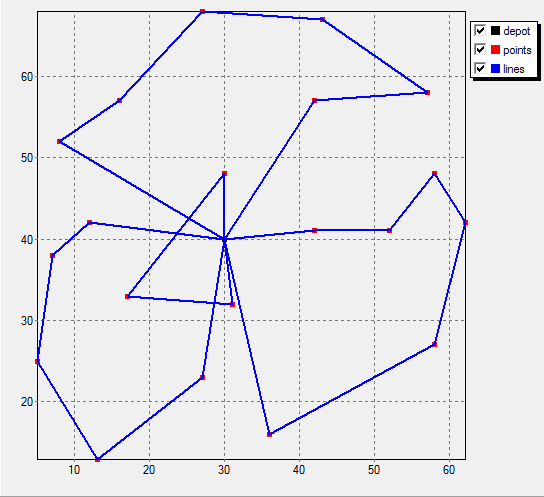
\includegraphics[width=\linewidth]{E021-04m-exact}
					\caption{Solución \emph{Exacta}}
				\end{subfigure} \
				\begin{subfigure}{.4\textwidth}
					\centering
					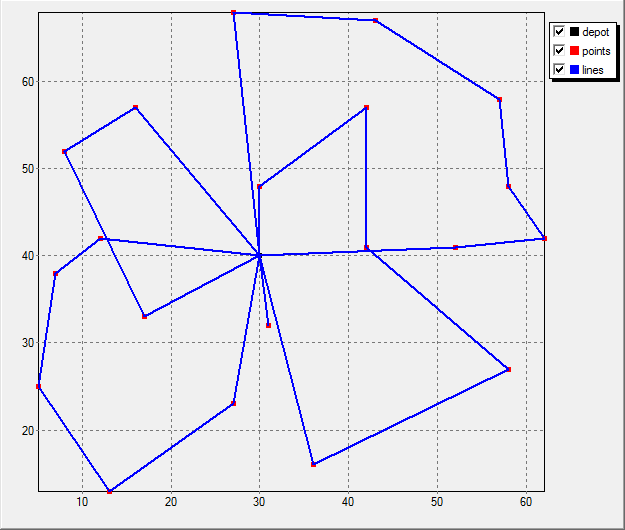
\includegraphics[width=\linewidth]{E021-04m-clarke-wright}
					\caption{Solución \emph{Clarke y Wright}}
				\end{subfigure}
				\caption{Resultados para el \emph{problema de rutado de vehículos capacitado (CVRP)} sobre el conjunto de datos \emph{E021-04m}}
				\label{fig:sol-e021-04m}
			\end{figure}

			\begin{table}[h]
				\centering
				\begin{tabu}{ | c | c | c | p{.58\linewidth} |}
					\hline
					\bfseries Método & \bfseries Vehículos  & \bfseries Distancia & \bfseries Caminos
					\csvreader[head to column names]{../results/csv/e021-04m.csv}{}
					{\\\hline\method&\vehicles&\distance&\path}
					\\\hline
				\end{tabu}
				\caption{Resultados para el \emph{problema de rutado de vehículos capacitado (CVRP)} sobre el conjunto de datos \emph{E021-04m}}
				\label{table:sol-e021-04m}
			\end{table}


		\subsection{E026-08m}

			\paragraph{}
			El conjunto de datos está formado por las coordenadas referidas a $26$ nodos, refiriendose el primero de ellos al nodo fuente u origen. Además se proporciona la demanda del resto de nodos junto con la capacidad máxima para cada vehículo ($48$ unidades) así como el número mínimo de ellos ($8$ vehículos) para resolver el problema. En este caso se ha resulto de manera exacta mediante la formulación descrita en la sección \ref{sec:exact_formulation} y de manera aproximada a partir de la heurística de \emph{Clarke-Wright} mediante la implementación que se muestra en la sección \ref{sec:clarke_wright}. Los resultados se muestran en la tabla \ref{table:sol-e026-08m}. Puesto que en este caso los datos se refieren a un problema euclídeo (con coordenadas) la representación gráfica de las soluciones se muestran en la figura \ref{fig:sol-e026-08m}.

			\begin{figure}[h]
				\centering
				\begin{subfigure}{.4\textwidth}
					\centering
					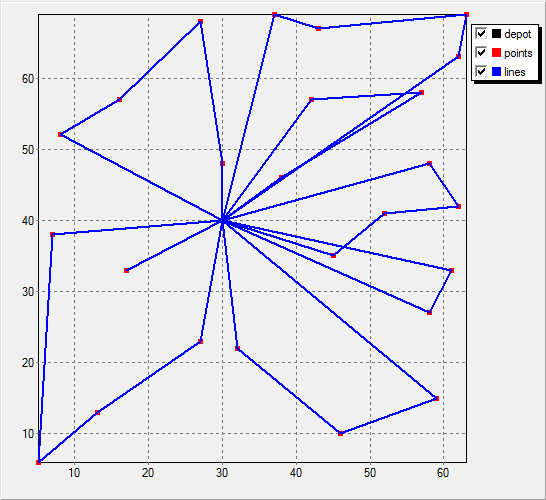
\includegraphics[width=\linewidth]{E026-08m-exact}
					\caption{Solución \emph{Exacta}}
				\end{subfigure} \
				\begin{subfigure}{.4\textwidth}
					\centering
					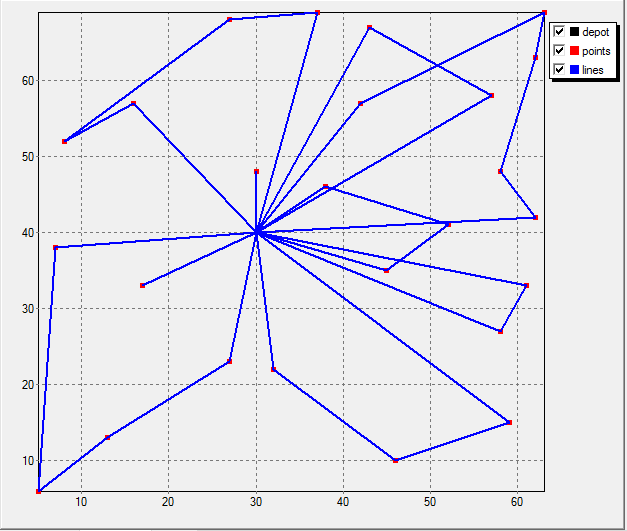
\includegraphics[width=\linewidth]{E026-08m-clarke-wright}
					\caption{Solución \emph{Clarke y Wright}}
				\end{subfigure}
				\caption{Resultados para el \emph{problema de rutado de vehículos capacitado (CVRP)} sobre el conjunto de datos \emph{E026-08m}}
				\label{fig:sol-e026-08m}
			\end{figure}

			\begin{table}[h]
				\centering
				\begin{tabu}{ | c | c | c | p{.58\linewidth} |}
					\hline
					\bfseries Método & \bfseries Vehículos  & \bfseries Distancia & \bfseries Caminos
					\csvreader[head to column names]{../results/csv/e026-08m.csv}{}
					{\\\hline\method&\vehicles&\distance&\path}
					\\\hline
				\end{tabu}
				\caption{Resultados para el \emph{problema de rutado de vehículos capacitado (CVRP)} sobre el conjunto de datos \emph{E026-08m}}
				\label{table:sol-e026-08m}
			\end{table}

		\subsection{E051-05e}

			\paragraph{}
			El conjunto de datos está formado por las coordenadas referidas a $51$ nodos, refiriendose el primero de ellos al nodo fuente u origen. Además se proporciona la demanda del resto de nodos junto con la capacidad máxima para cada vehículo ($160$ unidades) así como el número mínimo de ellos ($5$ vehículos) para resolver el problema. En este caso se ha resulto de manera exacta mediante la formulación descrita en la sección \ref{sec:exact_formulation} y de manera aproximada a partir de la heurística de \emph{Clarke-Wright} mediante la implementación que se muestra en la sección \ref{sec:clarke_wright}. Los resultados se muestran en la tabla \ref{table:sol-e051-05e}. Puesto que en este caso los datos se refieren a un problema euclídeo (con coordenadas) la representación gráfica de las soluciones se muestran en la figura \ref{fig:sol-e051-05e}.


			\begin{figure}[h]
				\centering
				\begin{subfigure}{.4\textwidth}
					\centering
					\includegraphics[width=\linewidth]{e051-05e-exact}
					\caption{Solución \emph{Exacta}}
				\end{subfigure} \
				\begin{subfigure}{.4\textwidth}
					\centering
					\includegraphics[width=\linewidth]{e051-05e-clarke-wright}
					\caption{Solución \emph{Clarke y Wright}}
				\end{subfigure}
				\caption{Resultados para el \emph{problema de rutado de vehículos capacitado (CVRP)} sobre el conjunto de datos \emph{E051-05e}}
				\label{fig:sol-e051-05e}
			\end{figure}

			\begin{table}[h]
				\centering
				\begin{tabu}{ | c | c | c | p{.58\linewidth} |}
					\hline
					\bfseries Método & \bfseries Vehículos  & \bfseries Distancia & \bfseries Caminos
					\csvreader[head to column names]{../results/csv/e051-05e.csv}{}
					{\\\hline\method&\vehicles&\distance&\path}
					\\\hline
				\end{tabu}
				\caption{Resultados para el \emph{problema de rutado de vehículos capacitado (CVRP)} sobre el conjunto de datos \emph{E051-05e}}
				\label{table:sol-e051-05e}
			\end{table}

		\subsection{E076-10e}

			\paragraph{}
			El conjunto de datos está formado por las coordenadas referidas a $76$ nodos, refiriendose el primero de ellos al nodo fuente u origen. Además se proporciona la demanda del resto de nodos junto con la capacidad máxima para cada vehículo ($140$ unidades) así como el número mínimo de ellos ($10$ vehículos) para resolver el problema. En este caso se ha resulto de manera exacta mediante la formulación descrita en la sección \ref{sec:exact_formulation} y de manera aproximada a partir de la heurística de \emph{Clarke-Wright} mediante la implementación que se muestra en la sección \ref{sec:clarke_wright}. Los resultados se muestran en la tabla \ref{table:sol-e076-10e}. Puesto que en este caso los datos se refieren a un problema euclídeo (con coordenadas) la representación gráfica de las soluciones se muestran en la figura \ref{fig:sol-e076-10e}.


			\begin{figure}[h]
				\centering
				\begin{subfigure}{.4\textwidth}
					\centering
					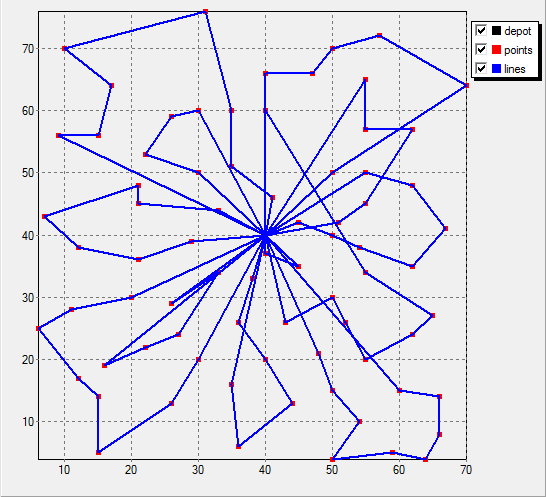
\includegraphics[width=\linewidth]{E076-10e-exact}
					\caption{Solución \emph{Exacta}}
				\end{subfigure} \
				\begin{subfigure}{.4\textwidth}
					\centering
					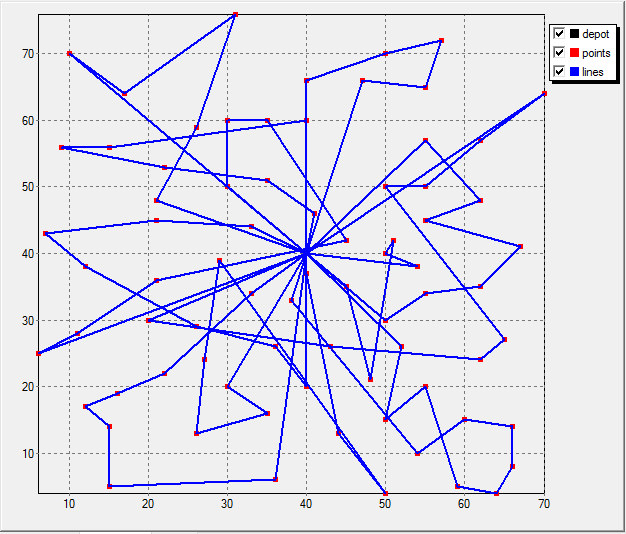
\includegraphics[width=\linewidth]{E076-10e-clarke-wright}
					\caption{Solución \emph{Clarke y Wright}}
				\end{subfigure}
				\caption{Resultados para el \emph{problema de rutado de vehículos capacitado (CVRP)} sobre el conjunto de datos \emph{E076-10e}}
				\label{fig:sol-e076-10e}
			\end{figure}

			\begin{table}[h]
				\centering
				\begin{tabu}{ | c | c | c | p{.58\linewidth} |}
					\hline
					\bfseries Método & \bfseries Vehículos  & \bfseries Distancia & \bfseries Caminos
					\csvreader[head to column names]{../results/csv/e076-10e.csv}{}
					{\\\hline\method&\vehicles&\distance&\path}
					\\\hline
				\end{tabu}
				\caption{Resultados para el \emph{problema de rutado de vehículos capacitado (CVRP)} sobre el conjunto de datos \emph{E076-10e}}
				\label{table:sol-e076-10e}
			\end{table}

%-----------------------------
%	BIBLIOGRAPHY
%-----------------------------
	\nocite{subject:mio}
	\nocite{garciparedes:mosel-examples}
	\bibliographystyle{alpha}
  \bibliography{bib/misc}

\end{document}
